\documentclass[10pt,landscape]{article}
\usepackage{multicol}
\usepackage{calc}
\usepackage{color}
\usepackage{ifthen}
\usepackage[landscape]{geometry}
\usepackage[ngerman]{babel}
\usepackage[utf8]{inputenc}
\usepackage{graphics}
\usepackage{listings}
\usepackage{verbatim}
\usepackage{multirow}
\usepackage{tikz}
\usetikzlibrary{arrows,automata}
\usepackage{alltt}
\usepackage{amsmath}   % allgemeine Mathe-Erweiterungen
\usepackage{amssymb}   % Symbole und Schriftarten
\usepackage{amsthm}    % erweiterte Theorem-Umgebungen

% This sets page margins to .5 inch if using letter paper, and to 1cm
% if using A4 paper. (This probably isn't strictly necessary.)
% If using another size paper, use default 1cm margins.
\ifthenelse{\lengthtest { \paperwidth = 11in}}
	{ \geometry{top=.5in,left=.3in,right=.5in,bottom=.5in} }
	{\ifthenelse{ \lengthtest{ \paperwidth = 297mm}}
		{\geometry{top=1cm,left=1cm,right=1cm,bottom=1cm} }
		{\geometry{top=1cm,left=1cm,right=1cm,bottom=1cm} }
	}

% Turn off header and footer
\pagestyle{empty}
 

% Redefine section commands to use less space
\makeatletter
\renewcommand{\section}{\@startsection{section}{1}{0mm}%
                                {-1ex plus -.5ex minus -.2ex}%
                                {0.5ex plus .2ex}%x
                                {\normalfont\large\bfseries}}
\renewcommand{\subsection}{\@startsection{subsection}{2}{0mm}%
                                {-1explus -.5ex minus -.2ex}%
                                {0.5ex plus .2ex}%
                                {\normalfont\normalsize\bfseries}}
\renewcommand{\subsubsection}{\@startsection{subsubsection}{3}{0mm}%
                                {-1ex plus -.5ex minus -.2ex}%
                                {1ex plus .2ex}%
                                {\normalfont\small\bfseries}}
% Special commands
\newcommand{\code}[1]{\texttt{#1}}

\makeatother

% Define BibTeX command
\def\BibTeX{{\rm B\kern-.05em{\sc i\kern-.025em b}\kern-.08em
    T\kern-.1667em\lower.7ex\hbox{E}\kern-.125emX}}

% Don't print section numbers
\setcounter{secnumdepth}{0}


\setlength{\parindent}{0pt}
\setlength{\parskip}{0pt plus 0.5ex}

% ----------------------------------------------------
% RouterEins(North/South)
\newcommand{\REN}{134.2.0.1/16}
\newcommand{\RES}{192.168.0.254/24}
% RouterZwei(North/South)
\newcommand{\RZN}{134.2.0.2/16}
\newcommand{\RZS}{10.0.0.254/8}
% RouterDrei(North/South)
\newcommand{\RDN}{10.0.8.1/21}
\newcommand{\RDS}{134.2.0.3/16}
% HostsNorth(East/West)
\newcommand{\HNE}{10.0.8.2/21}
\newcommand{\HNW}{10.0.8.3/21}
% HostSouth(North/South)
\newcommand{\HSN}{192.168.0.1/24}
\newcommand{\HSS}{192.168.0.2/24}
% HostSouthEast(East/West)
\newcommand{\HSEW}{10.0.0.1/8}
\newcommand{\HSEE}{10.0.0.2/8}
% Netze
\newcommand{\DSL}{192.168.0.0/24}
\newcommand{\FDDI}{134.2.0.0/16}
\newcommand{\ETH}{10.0.0.0/8}
\newcommand{\SETH}{10.0.8.0/21}

\newcommand{\Reins}{134.2.2.1}
\newcommand{\Rzwei}{134.2.3.1}
\newcommand{\Rdrei}{134.2.3.2}
\newcommand{\Rvier}{134.2.1.1}
\newcommand{\Rfunf}{134.2.1.2}
\newcommand{\Rsechs}{134.2.2.2}
\newcommand{\Rsieben}{134.2.4.1}
\newcommand{\Racht}{134.2.4.2}
\newcommand{\Rneun}{134.2.4.3}
\newcommand{\Rzehn}{134.2.1.3}
\newcommand{\Relf}{134.2.4.4}
% -----------------------------------------------------------------------

\begin{document}
\small
\raggedright
\begin{multicols}{3}


% multicol parameters
% These lengths are set only within the two main columns
%\setlength{\columnseprule}{0.25pt}
\setlength{\premulticols}{1pt}
\setlength{\postmulticols}{1pt}
\setlength{\multicolsep}{1pt}
\setlength{\columnsep}{2pt}

\begin{center}
     \Large{\textbf{GdI - CheatSheet}} \\
\end{center}

\section{Exercise 1}
\subsection{ISO/OSI - Schichtenmodell}
\begin{tabular}{l|l|l|l}
\multirow{3}{*}{Anw. } & \textcolor{red}{A}way! & 7 & Application \\
& \textcolor{red}{P}izza & 6 & Presentation \\
& \textcolor{red}{S}alami & 5 & Session \\
\hline
\multirow{4}{*}{Trans.} & \textcolor{red}{T}hrow & 4 & Transport \\
& \textcolor{red}{N}ot & 3 & Network \\
& \textcolor{red}{D}o & 2 & Data Link \\
& \textcolor{red}{P}lease & 1 & Physical \\
\end{tabular}
\subsubsection{Zuordnung OSI}
\begin{tabular}{l|l|l|l}
Prot. & Spec & Medium & OSI \\
\hline
& IP & & 3 \\
TCP & & & 4 \\
& & Koaxkabel & 1 \\
FTP & & & 7 \\
UDP & & & 4 \\
HTTP & & &  7 \\
VoIP & & & 7 \\
& & Sichtverb. & 1
\end{tabular}
\subsubsection{OSI-Ger\"ate}
\begin{tabular}{l|l|l}
Ger\"ate & Standard & OSI \\
\hline
& 802.11 & 2\\
Hub & & 1 \\
Switch & & 2 \\
Router & & 3\\
Gateway & & 3\\
& 802.3 & 2 (?)\\
& MobileIP & 3
\end{tabular}

\subsection{ARP}
\begin{tikzpicture}[shorten >=0.7pt,node distance=1.6cm,auto]
    \node[state]  (A)                       {A};
    \node[state]  (B) [below right of=A]    {B};
    \node[state]  (C) [right of=A]    {C};
    \path[->]   (A)     edge  node {} (B)
                (A)     edge  node {} (C)
                (B)     edge  node {} (C)
                ;
\end{tikzpicture}
A m\"ochte an B schicken, anschliessend C an A. Wie viele ARP-Pakete?
\begin{enumerate}
    \item A schickt ARP-Broadcast (B,C speichern ARP von A)
    \item B schickt ARP an A
\end{enumerate}
C hat die Adresse von A schon durch den Broadcast, daher werden nur zwei verschickt.

\subsection{IP-Adressen}
\subsubsection{Pr\"afix}
IP-Pr\"afix f\"ur 4 Subnetze mit 50 Hosts (A,B) und 200 Hosts (C,D):\\
\begin{itemize}
    \item[A,B] \textbf{/26} $2^26$ Bit f\"ur Netz, $2^6$ f\"ur Hosts (64)
    \item[C,D] \textbf{/24} $2^24$ Bit f\"ur Netz, $2^8$ f\"ur Hosts (255)
\end{itemize}
\subsubsection{IPs}
\begin{itemize}
    \item[A] Router-Port: 192.168.1.1/26, Hosts: 192.168.1.{2..51}
    \item[B] Router-Port: 192.168.2.1/26, Hosts: 192.168.2.{2..51}
    \item[C] Router-Port: 192.168.3.1/24, Hosts: 192.168.3.{2..201}
    \item[D] Router-Port: 192.168.4.1/24, Hosts: 192.168.4.{2..201}
\end{itemize}

\subsection{IP-Fragmentation}
Hmm...

\section{Exercise 2}
\subsection{Forwarding Table}
Die Hosts im DSL-Netzwerk m\"ussen \"uber den R1 geroutet werden,
da sie nicht nicht geswitched sind oder auf einem Bus kommunizieren. \\
\subsubsection{Trie}
\begin{tabular}{|c|c|}
    \hline
    Netzwerk & Next Hop  \\
    \hline\hline
    \multicolumn{2}{|c|}{Router 1}\\
    \hline
        \HSN &  $H1$ \\
        \HSS &  $H2$ \\
        \SETH & $R3$ \\
        \ETH & $R2$ \\
   \hline
\end{tabular}
\begin{tikzpicture}[shorten >=1pt,node distance=2cm,auto]

    \node[state]  (0)                                          {localhost};
    \node[state]  (1) [below right of=0,label=right:$192.168$]      {};
    \node[state]  (2) [below right of=1,label=below:$192.168.0.1$]  {};
    \node[state]  (3) [below of=1,label=below:$192.168.0.2$]    {};
    \node[state]  (4) [below left of=0,label=left:$134.2$]    {};
    \node[state]  (5) [below left of=4,label=below:$134.2.0.2$]    {};
    \node[state]  (6) [below of=4,label=below:$134.2.0.3$]    {};
    \node[state]  (7) [above of=0,label=left:$10.0$]    {};
    \node[state]  (8) [above right of=7,label=below:$10.0.0$]    {};
    \node[state]  (9) [above left of=7,label=below:$10.0.8$]    {};
    \node[state]  (10) [above right of=8,label=below:$10.0.0.1$]    {};
    \node[state]  (11) [below right of=8,label=below:$10.0.0.2$]    {};
    \node[state]  (12) [above left of=9,label=below:$10.0.8.2$]    {};
    \node[state]  (13) [below left of=9,label=below:$10.0.8.3$]    {};
    

  \path[->] (0)     edge  node {} (1)
            (1)     edge  node {} (2)
            (1)     edge  node {} (3)
            (0)     edge  node {} (4)
            (4)     edge  node {} (5)
            (4)     edge  node {} (6)
            (0)     edge  node {} (7)
            (7)     edge  node {} (8)
            (7)     edge  node {} (9)
            (8)     edge  node {} (10)
            (8)     edge  node {} (11)
            (9)     edge  node {} (12)
            (9)     edge  node {} (13)
            ;
\end{tikzpicture}

\subsection{Virtual Circuits}
\subsubsection{Hosts}
\begin{tabular}{|c|c|c|}
    \hline
    VCI & Inport & Outport  \\
    \hline\hline
    \multicolumn{3}{|c|}{Host \HSN}\\
    \hline
        L0 & - & \HSN \\
        L1 & - & \HSN \\
    \hline\hline
    \multicolumn{3}{|c|}{Host \HSS}\\
    \hline
        L4 & \HSS & - \\
    \hline\hline
    \multicolumn{3}{|c|}{Host \HSEW}\\
    \hline
        L1 & \HSEW & - \\
        L2 & \HSEW & - \\
    \hline\hline
    \multicolumn{3}{|c|}{Host \HSEE}\\
    \hline
        L2 & - & \HSEE \\
    \hline
\end{tabular}
\subsection{Router}

\begin{tabular}{|c|c|c|}
    \hline
    VCI & Inport & Outport  \\
    \hline\hline
    \multicolumn{3}{|c|}{R1}\\
    \hline
        L0 & \RZS & \REN \\
        L1 & \RZS & \REN \\
        L4 & \RZN & \RES \\
    \hline\hline
    \multicolumn{3}{|c|}{R2}\\
    \hline
        L1 & \RZN & \RZS \\
        L2 & \RZN & \RZS \\
        L3 & \RZS & \RZN \\
    \hline\hline
    \multicolumn{3}{|c|}{R3}\\
    \hline
        L0 & \RDS & \RDN \\
        L1 & \RDS & \RDN \\
        L4 & \RDN & \RDS \\
    \hline
    
\end{tabular}

\section{Exercise 3}
\subsection{Routing im INet}
\subsubsection{Interior Gateway Protocol}
Interior Gateway Protocol (IGP) ist eine Gattungsbezeichnung, die man auf jedes
Protokoll anwenden kann, das Informationen \"uber Wegewahl und Erreichbarkeit in
einem autonomen System verbreitet. IGP ist ein IP-Protokoll zum Austausch von
Routing-Informationen in autonomen Systemen.
Obwohl es keinen einzigen Standard f\"ur das IGP-Protokoll gibt,
ist das RIP-Protokoll das popul\"arste. Das IGP-Protokoll ist topologieunabh\"angig.
Da unterschiedliche Topologien und Netzwerke vorhanden sind,
gibt es mehrere Interior-Gateway-Protokolle.
Gateways k\"onnen gleichzeitig verschiedene Routing-Protokolle benutzen,
wenn sie die Verbindung zwischen 'autonomen Systemen' und einem \"ubergeordneten
Backbone-Netzwerk sind. Hierf\"ur stehen neben dem erw\"ahnten RIP-Protokoll
das Hello-Protokoll, das IGRP-Protokoll und das OSPF-Protokoll zur Verf\"ugung.\\

\subsubsection{Exterior Gateway Protocol}
Das Exterior Gateway Protocol (EGP) ist auf der Vermittlungsschicht des
OSI-Referenzmodells angesiedelt und baut auf dem IP-Protokoll auf.
Das EGP wird zur Kommunikation zwischen Routern benutzt und dient dem Verbund
mehrerer komplexer Netze, die in sich eine abgeschlossene Welt bilden und nur
gelegentlich mit anderen Netzen kommunizieren. Ein solches Netz wird in
TCP/IP-Terminologie als autonomes System  bezeichnet. Es bildet mit anderen
autonomen Systemen im Verbund ein 'Netz von Netzen'. In jedem autonomen System
des Netzwerkverbundes wird nun mindestens ein Edge Router (ER) als
Exterior-Gateway eingerichtet, der das autonome System mit den
anderen autonomen Systemen verbindet.\\

\subsubsection{Abgrenzung}
EGP arbeitet mit \textbf{Distance Vector Routing} in dem es die Informationen
seiner Nachbarn zur Erreichbarkeit anderer Netze sammelt und Informationen an seine
eigenen Nachbarn weitergibt.\\
Ferner ist es limitiert auf baumartig aufgebaute Netze.
Hierdurch kann es ab einer Gewissen Netzkomplexit\"at schlichtweg nicht mehr skalieren
und ist damit mittlerweile obsolet.
IGP hingegen bezeichnet eine ganze Familie von Routingprotokollen, das
popul\"arste ist das RIP-Protokoll.

\subsubsection{Link State Routing}
Beim LSR wird eine Konfigurations\"anderung an das komplette Netz geschickt. \\
\"Andert sich ein Link, so wird diese Information direkt an alle
beiteiligten Hosts geschickt. \\

\subsubsection{Distance Vector Routing}
Beim DVR senden sich die Router gegenseitig Informationen \"uber die von ihnen aus
erreichbaren Hosts.\\
Initial versendet jeder Host im Grunde nur, dass er sich selbst \"uber sich selbst erreichen kann.\\
Darauf aufbauend, kann ein Nachbarhost nun die Information in seine Routingtabelle aufnehmen.\\
Diese Information sendet er einen Hop weiter an den n\"achsten Host.\\
So baut sich nach einigen Informationsaustauschen eine Tabelle mit der Erreichbarkeit des kompletten Netzwerk auf.

\subsection{3.1.3 Protokollzuorndung}
\begin{itemize}
    \item \textbf{RIP} Ein Protokoll der IGP-Familie und nutzt DistanceVectorRouting
    \item \textbf{OSPF} OSPF (Link-State-Routing) ist ein dynamisches Routing-Protokoll innerhalb eines autonomen Systems. \\
        Es hat das Routing Information Protocol (RIP) als Standard-Interior Gateway Protocol (IGP) abgel\"ost
    \item \textbf{BGP} Ein DistanceVektorRouting-Protokoll der IGP-Familie 
\end{itemize}


\subsection{Dijkstra}
Die Grundidee des Algorithmus ist es, immer derjenigen Kante zu folgen,
die den k\"urzesten Streckenabschnitt vom Startknoten aus verspricht. \\
Andere Kanten werden erst dann verfolgt, wenn alle k\"urzeren Streckenabschnitte beachtet wurden.
Dieses Vorgehen gew\"ahrleistet, dass bei Erreichen eines Knotens kein k\"urzerer Pfad zu ihm existieren kann. \\
Eine einmal berechnete Distanz zwischen dem Startknoten und einem erreichten Knoten wird nicht mehr ge\"andert.
Dieses Vorgehen wird fortgesetzt, bis die Distanz des Zielknotens berechnet wurde (single-pair shortest path)
oder die Distanzen aller Knoten zum Startknoten bekannt sind (single-source shortest path).
\tiny
\begin{tabular}{l|l|l}
\textbf{Step}   & \textbf{confirmed}    & \textbf{tentative} \\
1   & (I,0,-)           & (D,5,D);(G,1,G);(E,5,E);(H,3,H) \\
2   & (I,0,-);(G,1,G)   & (D,3,G);(E,5,E);(H,3,H) \\
3   & (I,0,-);(G,1,G);(D,3,G)   & (E,5,E);(H,3,H);(B,7.5,D) \\
4   & (I,0,-);(G,1,G);(D,3,G);(H,3,H)   & (E,5,E);(B,7.5,D);(F,11,H) \\
\end{tabular}

\subsection{Bellman-Ford}
\small
Anders als beim Algorithmus von Dijkstra, dem bekanntesten Verfahren zur Suche nach k\"urzesten Wegen in Graphen,
k\"onnen die Gewichte der Kanten auch negativ sein, allerdings d\"urfen keine Kreise negativen Gewichtes vorkommen. \\
Falls es negative Kreise gibt, findet der Algorithmus nicht zu jedem Knoten den k\"urzesten Weg.
Es ist jedoch m\"oglich, mit dem Algorithmus das Vorhandensein von Kreisen negativen Gewichtes zu erkennen.

\newpage
\section{Exercise 4}
\subsection{OSPF}
\subsubsection{Aufteilen des Netzes in drei Regionen}
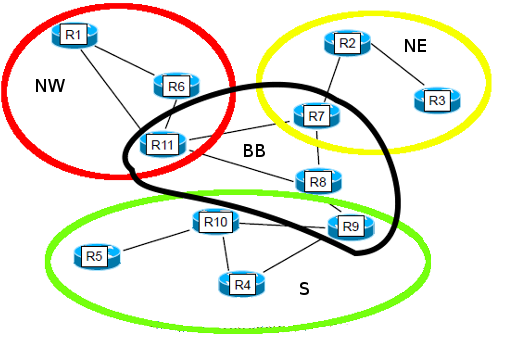
\includegraphics[scale=0.5]{a.png}
\subsubsection{Adresszuweisung}
\begin{tabular}{|l|l|l|} 
\hline
Router& Group & Adress\\
\hline \hline
1 & NW & \Reins \\ 
\hline
2 & NE & \Rzwei \\ 
\hline
3 & NE & \Rdrei \\ 
\hline
4 & S & \Rvier \\ 
\hline
5 & S & \Rfunf \\ 
\hline
6 & NW & \Rsechs \\ 
\hline
\textbf{7} & \textbf{BB} & \textbf{\Rsieben}\\ 
\hline
8 & BB & \Racht \\ 
\hline
\textbf{9} & \textbf{BB} & \textbf{\Rneun}\\ 
\hline
10 & S & \Rzehn \\ 
\hline
\textbf{11} & \textbf{BB} & \textbf{\Relf}\\ 
\hline
\end{tabular}

\subsubsection{Routing Tabellen der ABRs}

\paragraph{R7 (134.2.4.1)}
\begin{tabular}{|l|l|l|} 
\hline
IP& via & Distance\\
\hline \hline
134.2.3.1 (R2) & self & 1\\ 
134.2.3.2 (R3) & 134.2.3.1 (R2) & 2\\
134.2.4/24 (Area NW) & 134.2.4.4 (R11) & 2\\
134.2.1/24 (Area S) & 134.2.4.2 (R8) & 3\\
134.2.4.4 (R11) & self & 1\\
134.2.4.2 (R8) & self & 1\\
134.2.4.3 (R9) & 134.2.4.2 (R8) & 2\\
\hline
\end{tabular}

\subsubsection{Vorteile OSPF}
\begin{itemize}
\item Ein Router in einer Area muss nur die Wege zu Routern in derselben Area kennen. Der genaue Aufbau 
    anderer Areas, auch der Backbone-Area, ist ihm nicht bekannt. Routings in diese Bereiche gehen "uber
    den ABR. Dem ABR gen"ugt es, die \textit{Richtung} 
    aller Areas zu kennen. Dadurch wird der Routing-Traffic minimiert.
\item Im Gegensatz zum Routing-Information-Protocol garantiert OSPF ein \textit{schleifenfreies} Routing.
\item Die Unterteilung in Areas macht die Wartung des gesamten Netzes sehr einfach. Da die genaue Topologie
einer Area dem restlichen Netzwerk unbekannt ist, k"onnen die Einzelnetzwerke in ihrem Aufbau ver"andert werden,
ohne dass das restliche Netzwerk dar"uber informiert werden muss. Dadurch ist OSPF vor allem f"ur sehr grosse Netze
geeinget, die erweiterbar bleiben sollen.
\end{itemize}

\subsubsection{Verbindung Backbone Area,warum?}
Routing in \textit{fremde} Areas gehen bei OSPF immer "uber die ABRs, die sowohl zum eigenen Bereich als auch
zum Backbone verbunden sind. Alle Routinginformationen, die zwischen Areas ausgetauscht werden, gehen "uber den Backbone. 
Sollte in OSPF also eine Area (entgegen der Klassifikation) "uber keine Verbindung zum Backbone verf"ugen, w"urde nur Routing 
innerhalb der eigenen Area m"oglich.


\subsection{Effect of congestion}

\subsubsection*{Maximum relative send rate}
Jeder Link hat die Bandbreite B, und jeder Link h"alt 2 Verbindungen. Trivialerweise ist die maximale relative send rate 0.5 .
\subsubsection{Loss ratio}
Es gilt \[R = x*B\] \[\Rightarrow R_{loss} = (x - x_0) * B\]
Somit \[p = \frac{R_{loss}}{R} = \frac{(x-x_0) * B}{x*B} = \frac{x-x_0}{x}\]

\subsubsection{zusammenhang y/R und x}

\section{Exercise 5}
\subsection{BGP-advertisements}
\subsubsection{advertising}
UPDATE-Nachrichten (Folie 184)
\begin{itemize}
    \item $AS1 \to AS2: 134/8:AS1;R1$
    \item $AS2 \to AS3: 134/8:AS2,AS1;R2$
    \item $AS2 \to AS5: 134/8:AS2,AS1;R2$
    \item $AS3 \to AS4: 134/8:AS3,AS2,AS1;R3$
    \item $AS3 \to AS5: 134/8:AS3,AS2,AS1;R3$
    \item $AS4 \to AS5: 134/8:AS4,AS3,AS2,AS1;R4$
    \item $AS5 \to AS6: 134/8:[[AS5],AS4],AS3,AS2,AS1;R5$ 
    \item $AS5 \to AS4: 138/8:[AS3],AS2,AS1;R5$ 
    \item $AS5 \to AS3: 138/8:AS2,AS1;R5$
    \item $AS4 \to AS3: 138/8:AS4,AS5,AS2,AS1;R4$
\end{itemize}
\subsubsection{Wie viele Routen kennt R5, welche announced er zu R6?}
\begin{itemize}
    \item Der innere Knoten R5 kennt die Routen \"uber A2,3,4
    \item Wie in 5.1 anounced er einen Weg der f\"ur ihn optimal erscheint. Evtl. nach Kostenaspekt, oder Bandbreite, Stabilit\"at, etc.
\end{itemize}
\subsubsection{Route bricht weg}
WITHDRAW-Nachrichten (Folie 186)
\begin{itemize}
    \item $AS2 \to AS3: 134/8$
    \item $AS2 \to AS5: 134/8$
    \item $AS3 \to AS4: 134/8$
    \item $AS3 \to AS5: 134/8$
    \item $AS4 \to AS5: 134/8$
    \item $AS5 \to AS6: 134/8$
\end{itemize}
\subsubsection{Links wieder da, anderer Links brechen weg}
\begin{itemize}
    \item Da es in dem kostenpflichten Links nur AS2 und AS5 betrifft, werden dort keine WITHDRAWS verschickt.\\
    Sollte AS5 zu AS6 einen Pfad mit dieser Route anounced haben, dann wird er ein UDATE mit einer alternativen Route schicken.
    \item R3 w\"urde den prefix bei R5 und R4 WITHDRAWen. R3 rekonfiguriert seine Route aus den schon bekommenen Inforamtionen und schickt nun \"uber R5.
\end{itemize}

\subsection{BGP - eBGP/iBGP}
Mehrere AS\_X-Teilnetze, die Frage ist, wie welcher Router in den Netzen die Routen zu den anderen lernt.\\
Das Ding ist zu schauen, wie viele Hops gebraucht werden, bis die Information von einem zum anderen hoppelt.\\
Wer zuerst kommt, der malt dann auch zuerst.
\subsubsection{Informationswege Teilrouter werden abgefragt}
\begin{enumerate}
    \item Erst breitet sich die Information in AS4 \"uber RIP aus.
    \item 4c berichtet \"uber eBGP an 3c
    \item 3c nutzt innerhalb AS3 OSPF (3a)
    \item AS3 teilt AS1 (dem Router 1c) \"uber eBGP das Prefix mit    
\end{enumerate}
\subsubsection{What interface of 1d will be configured to route the prefix x?}
IF1, da der Router 1a die Information eher hat als 1b.
\subsubsection{Welches Interface von RouterX?}
Die Hopanzahl zu 1b von 4a ist 3, zu 1a ist sie 6.\\
Somit ist davon auszugehen, dass 1b die Information eher an 1d schicken wird und somit IF2 konfiguriert wird.
\subsubsection{Interface?}
Da die Netze alle shared-cost verbunden sind, wird nach einer Heuristik entschieden.\\
Am wahrscheinlichsten w\"are die Entscheidung an hand der Anzahl der Hops zu treffen, dann w\"are IF1 die beste Wahl.\\
Evtl. k\"onnte der andere Pfad jedoch mit einer besseren Verbindung werben, dann ist evtl. IF2 besser.
Ohne Zusatzinformationen w\"urde ich jedoch IF1 favorisieren.

\section{Exercise 6}
\subsection{Forwarding and routing tables}

\subsection{Stop'N'Wait,GoBackN,Selective Repeat}
\begin{itemize}
    \item 10 Gbit/s Netz
    \item packet size 4000byte
    \item rtt 200ms
\end{itemize}
\subsubsection{transmit-Time des Pakets}
Es gilt $d_{saw} = \frac{L}{R} + t_{rtt}$, wobei $L$ die Paketl\"ange ist,
$R$ die \"Ubertragungsgeschwindigkeit und $t_{rtt}$ die
\textit{round-travel-time}. Im vorliegen Fall wird die
\"Ubertragungsdauer der ACK-Pakete vernachl\"assig, somit gilt
$d_{saw} = \frac{4000*8 bit}{10^{10} bps} + 20ms = 20,0032ms$
\subsubsection{utilization}
Es gilt $U_{saw} = \frac{L/R}{t_{rtt} + L/R}$ \\
$\Rightarrow U_{saw} = \frac{0,0032ms}{20,0032ms} = 1,59974 * 10^{-4}$

\subsubsection{Effektiver Druchsatz}
Effektiv werden f\"ur die \"Ubertragung von 4000 byte 20,0032ms ben\"otigt. \\
Also: $R_{saw} = \frac{4000*8 bit}{20,0032ms} = 1599b/ms = 1.599.000b/s$

\subsubsection{Fenstergr\"osse f\"ur 90 $U_{saw}$}
$\dfrac{N * L/R}{rtt + L/R} = 0.9$
$N = 5626$

\subsubsection{Warum ist GBN uneffizient bei Paketverlusten?}
Bei wiederholten Paketverlusten kommt es bei GBN zur mehrfachen \"Ubertragen von Paketen.
Angenommen, Paket $x$ kommt \"uberhaupt nicht an. Der Sender schickt weiterhin Pakete im Fenster n,
bis der Timeout f\"ur die ACK-R\"uckmeldung f\"ur Paket 3 beim Sender eintritt.
Nun wird Paket 3 und \textbf{alle} anderen Pakete im Fenster nochmal geschickt.

\subsubsection{Wie kann GBN diesbez\"uglich verbessert werden?}
Dieser Nachteil kann z.B. durch einen Buffer beim Empf\"anger behoben werden.
Wird ein fehlerhaftes Paket empfangen, werden trotzdem weiterhin Pakete vom Sender angenommen.
Bei einem ACK-Timeout schickt der Sender nun nur das \textbf{\"alteste} noch nicht best\"atigte Paket
nochmal. Der Empf\"anger f\"ugt dieses in seinen Buffer ein und kann die Pakete dann komplett weiterleiten.


\subsection{Selective Repeat}
\subsubsection{Fenster $[k;k+N-1]$ mit N in-flights,welche SequenzNR?}
Paket Nummer $k-1$ wurde auf Empf\"angerseite empfangen und best\"atigt.
Somit wartet der Empf\"anger auf die Pakete ab der Nummer $k$.

\subsubsection{gehen alle in-flights verloren (data/ack), wieviele SequenzNR werden zur Zuordnung ben\"otigt?}
Die Anzahl der Sequenznummern sollte so gross sein, wie die Fenstergr\"osse. \\
Durch den Buffer beseht hier die Gefahr, dass ein Paket verloren geht und die Sequenznummer wiederverwendet wird, bevor der Timeout zuschl\"agt.\\
So w\"urde der Empf\"anger die Sequenznummer des zweiten Pakets best\"atigen und der Sender w\"urde denken es handelt sich um die Best\"atigung des ersten Paketes.

\subsubsection{Wieviele SeqNr brauch der GBN zum Erfolg?}
Da das Problem aus 6.3.2 nicht auftreten kann, muss der Sequenznummer-Menge nur so gross sein, wie Pakete innerhalb des Timeouts geschickt werden k\"onnen.
$Timeout / RTT $

\subsubsection{Wenn das Netz die Reinfolge verdreht, \"andert das was?}
\paragraph{SR} Bei SR haben wir schon die maximale Sequenznummer-Menge definiert, hier \"andert sich nichts. \\
\paragraph{GBN} Durch die extrem vergr\"osserten Timeouts kann nicht mehr festgestellt werden, welches Paket gerade angekommen ist, sollten die Nummer weiderverwendet werden.\\
Daher gilt nun auch hier als Sequenznummer-Menge die Fenstergr\"osse.

\newpage
\section{Exercise 7}
\subsection{TCP time to receive data}
\textbf{Ablauf:}\\
SYN $ \xrightarrow{SYN-ACK}$ ACK + S $\rightarrow$ 2 S $\rightarrow$ 4 S $\rightarrow$ 8 S $\rightarrow$ done\\
Jeder $\rightarrow$ entspricht einer RTT. Also gibt es 5 RTTs. Transportdauer betr"agt $\frac{15S}{R}$.
\[ 5\ RTT + \frac{15S}{R} \]
\begin{align*}
	1.\quad & \frac{S}{R} > RTT:& 
		&\frac{20S}{R} > 5\ RTT + \frac{15S}{R} > 20\ RTT\\
	2.\quad & RTT > \frac{3S}{R}:&
		&10\ RTT > 5\ RTT + \frac{15S}{R} > \frac{30S}{R}\\
	3.\quad & \frac{3S}{R} > RTT > \frac{2S}{R}:& 
		& \frac{30S}{R} > 5\ RTT + \frac{15S}{R} > \frac{25S}{R}
\end{align*}
\subsection{TCP loss rate}
\subsubsection{Beweis LossRate irgendwas}
\subsubsection{Noch nen Beweis von 'rate' aus n"achster Aufg...}
\subsubsection{VerlustWahr. 1500byte,100ms RTT, 10Gbit/s Link?}
\paragraph*{gegeben:} $MMS=1500\ Byte,\ RTT=100ms,\ rate=10 \frac{GBit}{s}$
\begin{align*}
	rate &= \frac{1.22 \cdot MMS}{RTT \cdot \sqrt{L}}\\
	rate \cdot RTT &= \frac{1.22 \cdot MMS}{\sqrt{L}}\\
	\frac{rate \cdot RTT}{1.22 \cdot MMS} &= \frac{1}{\sqrt{L}}\\
	L &= \left(\frac{1.22 \cdot MMS}{rate \cdot RTT}\right)^2 \\
	L &= \left(\frac{1.22 \cdot 1500\ Byte}{1.25 \frac{GByte}{s} \cdot 0.1s}\right)^2 \\
	L &= 1.8590129435835934e-10
\end{align*}

Wenn die Wahrscheinlichkeit h"oher ist, dann wir der Datendurchsatz sinken, da die Windowsize
"ofter kleiner wird und mehrmals die gleichen Daten gesendet werden m"ussen.

\section{Exercise 8}
\subsection{DNS-Verkehrsmodelle}
\subsubsection{Anzahl $N_k$ Domains auf k, k=0 ist root}
Es handelt sich um einen vollst"andigen Baum mit 10 Kindern auf jeder Ebene.
Jeder Knoten hat also 10 Nachfolger.\\
Auf Ebene 0 gibt es einen Knoten, auf der N"achsten Ebene 10, auf der darauffolgenden $10 \cdot 10$, also 100, 
darauffolgend $10 \cdot 100$ (jeder der hundert hat 10 Kinder) usw.
Auf der Ebene k gibt es also $10^k$ Dom"anen.

\subsection{Ebene4-DNS lokaler DNS;iterative Anfragen,mathematischen Ausdruck?}
Der lokale Nameserver kennt die obersten m Nameserver bereits, d.h. seine erste Anfrage beginnt gerade bei dem m-ten Nameserver. 
Somit muss er $k-m+1$ Anfragen leisten, um an die IP Adresse zu kommen. 
Somit ist die Zeit f"ur die Anfragedauer gerade $= (k-m+2) \cdot t$
(W"are $m = 0$, m"usste er jedoch $2 \cdot k$ Anfragen starten, da er sich erst den Baum hocharbeiten m"usste, 
was man nicht machen muss, wenn er zumindestens die Wurzel kennen w"urde, also $m > 0$ ist)


\subsubsection{Antwortzeiten 100ms und m=1,2,3,4,5}
\begin{align*}
    t &= 100ms\\
    m &= 1:  Zeit = k*t = 5*100ms = 500 ms\\
    m &= 2:  Zeit = k*t = 4*100ms = 400 ms\\
    m &= 3:  Zeit = k*t = 3*100ms = 300 ms\\
    m &= 4:  Zeit = k*t = 4*100ms = 200 ms\\
    m &= 5:  Zeit = k*t = 5*100ms = 100 ms
\end{align*}


\subsubsection{Wenn DNS rekursiv..}

\paragraph{Mathematischer Ausdruck?}\ \\
Bei der Rekursiven Variante muss man erst k Ebenen nach oben gelangen, dann wieder k Ebenen nach unten, 
nun schickt man die Antwort zur"uck, muss also wieder k Ebenen nach oben und wieder k Ebenenen nach unten.
Somit gilt f"ur die Zeit: Zeit = $4 \cdot k \cdot t$

\paragraph{Zeiten f\"ur 100ms und k=0,1,2,3,4} \ \\
\begin{align*}
    k = 0: 4 \cdot 0 \cdot t &= 0\\
    k = 1: 4 \cdot 1 \cdot 100ms  &= 400 ms\\
    k = 2: 4 \cdot 2 \cdot 100ms  &= 800 ms\\
    k = 3: 4 \cdot 3 \cdot 100ms  &= 1200 ms\\
    k = 4: 4 \cdot 4 \cdot 100ms  &= 1600 ms\\
\end{align*}


\paragraph{Wie lange, wenn der lokale DNS die oberen 1,2,3,4,5 Ebenen schon kennt?} \ \\ 
Kennt man die m obersten Nameserver, muss man nicht mehr zweimal nach unten und zweimal nach oben steigen, 
sondern jeweils nur einmal, und zwar $k-m+2$ mal oft. 
Also gilt: Zeit = $(k - m + 2) \cdot 2 \cdot t$. Somit ergibt sich 
(f"ur $k = 4$ angenommen, ist aus Aufgabenstellung nicht eindeutig ersichtlich)
\begin{align*}
    m = 1: \text{ Zeit } = (k - m + 2) \cdot 2 = 10 \cdot 100\ ms = 1000\ ms\\    
    m = 2: \text{ Zeit } = (k - m + 2) \cdot 2 = 20 \cdot 100\ ms = 2000\ ms\\
    m = 3: \text{ Zeit } = (k - m + 2) \cdot 2 = 30 \cdot 100\ ms = 3000\ ms\\
    m = 4: \text{ Zeit } = (k - m + 2) \cdot 2 = 40 \cdot 100\ ms = 4000\ ms\\
    m = 5: \text{ Zeit } = (k - m + 2) \cdot 2 = 50 \cdot 100\ ms = 5000\ ms
\end{align*}

\newpage
\subsubsection{DNS-Last bei verschiedenen Modellen}
\begin{itemize}
    \item[A] Anfragen gleichverteilt
    \item[B] 50\% werden lokal, der Rest gleichverteilt.
\end{itemize}
Von den lokalen Nameservern werden insgesamt $10^{n+1}$ Anfragen generiert, 
f"ur $n = 4$ haben wir also $10^5$ Anfragen pro Sekunde.
\paragraph{Verkehrsmodell A:}
Sind die Anfragen gleichverteilt, bekommt auf Ebene $k$ ein Nameserver $10^{k+1}$ Anfragen, also gilt:
\begin{align*}
    k = 4:\qquad & 10^5 \text{ Anfragen}\\
    k = 3:\qquad & 10^4 \text{ Anfragen}\\
    k = 2:\qquad & 10^3 \text{ Anfragen}\\
    k = 1:\qquad & 10^2 \text{ Anfragen}\\
    k = 0:\qquad & 10^1 \text{ Anfragen}
\end{align*}


\paragraph{Verkehrsmodell B:}  50\% aller Anfragen bleiben auf einer Ebene Lokal
\begin{align*}
    k = 4:\qquad &   10^5 \text{ Anfragen}\\
    k = 3:\qquad & 50000 \text{ Anfragen}\\
    k = 2:\qquad & 25000 \text{ Anfragen}\\
    k = 1:\qquad & 12500 \text{ Anfragen}\\
    k = 0:\qquad &  6500 \text{ Anfragen}  
\end{align*}
4
\subsection*{6.}

\paragraph{Verkehrsmodell A:}
\begin{align*}
    k = 4:\qquad & 10^5 \text{ Anfragen}\\
    k = 3:\qquad & 10^4 \text{ Anfragen}\\
    k = 2:\qquad & 10^3 \text{ Anfragen}\\
    k = 1:\qquad & 10^2 \text{ Anfragen}\\
    k = 0:\qquad & 10^1 \text{ Anfragen}
\end{align*}

\paragraph{Verkehrsmodell B:} 
Nur beim lokalem Nameserver schlagen alle Anfragen auf.
Dieser kann diese dann aber direkt sinnvoll verteilen.
\begin{align*}
    k = 4:\qquad &   10^5 \text{ Anfragen}\\
    k = 3:\qquad & 25000 \text{ Anfragen}\\
    k = 2:\qquad & 12500 \text{ Anfragen}\\
    k = 1:\qquad & 6500 \text{ Anfragen}\\
    k = 0:\qquad &   6500 \text{ Anfragen} \\   
\end{align*}

\subsection*{7.}

\paragraph{Verkehrsmodell B:} 
\begin{align*}
    k = 4:\qquad & \frac{10^5}{10^4} = 10 \text{ Anfragen}\\
    k = 3:\qquad & \frac{10^4}{10^3} = 10\text{ Anfragen}\\
    k = 2:\qquad & \frac{10^3}{10^2} = 10 \text{ Anfragen}\\
    k = 1:\qquad & \frac{10^2}{10} = 10 \text{ Anfragen}\\
    k = 0:\qquad & 10 \text{ Anfragen}
\end{align*}

\paragraph{Verkehrsmodell B:} 
\begin{align*}
    k = 4:\qquad & \frac{10^5}{10^4} \text{ Anfragen}\\
    k = 3:\qquad & \frac{50000}{10^3} \text{ Anfragen}\\
    k = 2:\qquad & \frac{25000}{10^2} \text{ Anfragen}\\
    k = 1:\qquad & \frac{12500}{10} \text{ Anfragen}\\
    k = 0:\qquad &  6500 \text{ Anfragen}  
\end{align*}


\subsection{NSLookup}

\end{multicols}
\end{document}
